%\documentclass[mathserif]{beamer}
\documentclass[handout]{beamer}
%\usetheme{Goettingen}
\usetheme{Warsaw}
%\usetheme{Singapore}
%\usetheme{Frankfurt}
%\usetheme{Copenhagen}
%\usetheme{Szeged}
%\usetheme{Montpellier}
%\usetheme{CambridgeUS}
%\usecolortheme{}
%\setbeamercovered{transparent}
\usepackage[english, activeacute]{babel}
\usepackage[utf8]{inputenc}
\usepackage{amsmath, amssymb}
\usepackage{dsfont}
\usepackage{graphics}
\usepackage{cases}
\usepackage{graphicx}
\usepackage{pgf}
\usepackage{epsfig}
\usepackage{amssymb}
\usepackage{multirow}	
\usepackage{amstext}
\usepackage[ruled,vlined,lined]{algorithm2e}
\usepackage{amsmath}
\usepackage{epic}
\usepackage{epsfig}
\usepackage{fontenc}
\usepackage{framed,color}
\usepackage{palatino, url, multicol}
\usepackage{listings}
%\algsetup{indent=2em}
\newcommand{\factorial}{\ensuremath{\mbox{\sc Factorial}}}
\newcommand{\BIGOP}[1]{\mathop{\mathchoice%
{\raise-0.22em\hbox{\huge $#1$}}%
{\raise-0.05em\hbox{\Large $#1$}}{\hbox{\large $#1$}}{#1}}}
\newcommand{\bigtimes}{\BIGOP{\times}}
\vspace{-0.5cm}
\title{Data Exploration}
\vspace{-0.5cm}
\author[Felipe Bravo Márquez]{\footnotesize
%\author{\footnotesize  
 \textcolor[rgb]{0.00,0.00,1.00}{Felipe José Bravo Márquez}} 
\date{ \today }


\begin{document}
\begin{frame}
\titlepage


\end{frame}


%%%%%%%%%%%%%%%%%%%%%%%%%%%






\begin{frame}{Exploratory Data Analysis}
\scriptsize{
\begin{itemize}
 \item Exploratory Data Analysis or (EDA) encompasses a set of techniques to quickly understand the nature of a data collection or \textbf{dataset}.
 
 \item It was proposed by the statistician John Tukey.
 
 \item It is based mainly on two criteria: \textbf{summary statistics} and \textbf{data visualization}.
 
 \item In this class you will see both types of techniques, in addition to their application in R for some toy datasets.
\end{itemize}

}

\end{frame}

\begin{frame}{El dataset Iris}
\scriptsize{
\begin{itemize}
 \item Trabajaremos con un dataset muy conocido en análisis de datos llamado \textbf{Iris}.
 \item El dataset se compone de 150 observaciones de flores de la planta iris. 
 \item Existen tres tipos de clases de flores iris: \textbf{virginica}, \textbf{setosa} y \textbf{versicolor}.
 \item Hay 50 observaciones de cada una.
\item Las variables o atributos que se miden de cada flor son:

\begin{enumerate}
\scriptsize{
 \item El tipo de flor como variable categórica.
 \item El largo y el ancho del pétalo en cm como variables numéricas.
 \item El largo y el ancho del sépalo en cm como variables numéricas.
  }
\end{enumerate}

 
\end{itemize}


\begin{figure}[h!]
	\centering
	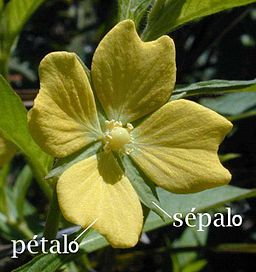
\includegraphics[scale=1.2]{pics/petalosepalo.jpg}
	
	
\end{figure}

}

\end{frame}

\begin{frame}[fragile]{El dataset Iris}
\scriptsize{


 \begin{figure}[h!]
\begin{center}
\begin{tabular}{ccc}
 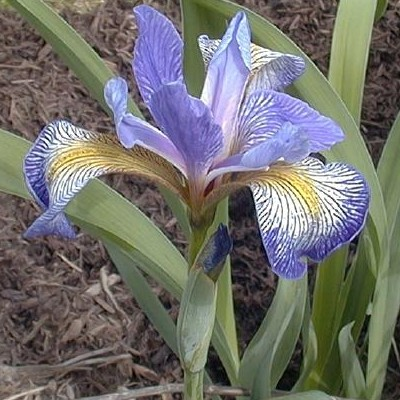
\includegraphics[width=3cm]{pics/virginica.jpg}
&
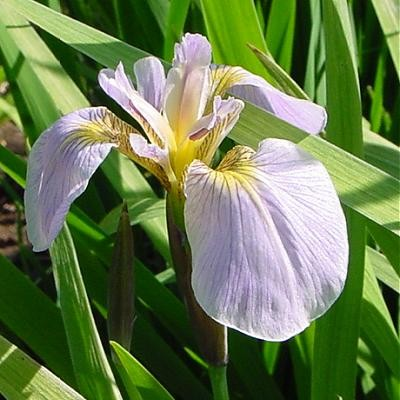
\includegraphics[width=3cm]{pics/setosa.jpg}
&
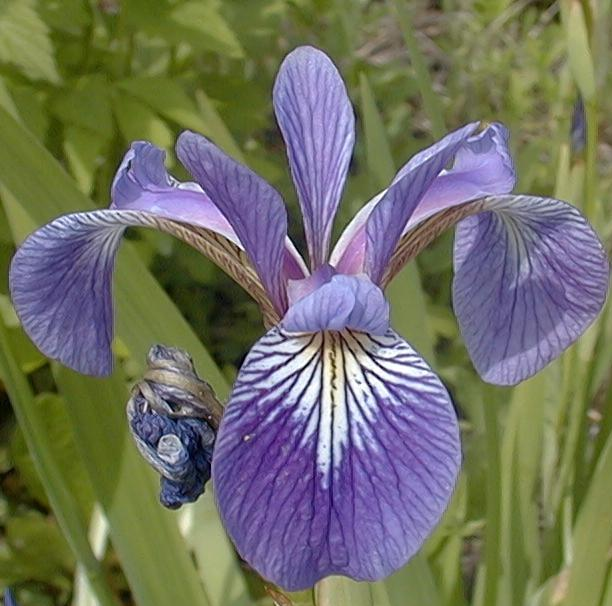
\includegraphics[width=3cm]{pics/versicolor.jpg}
\end{tabular}
\caption{Virginica - Setosa - Versicolor}
\end{center}
\end{figure}

\begin{itemize}
 \item El dataset se encuentra disponible en R:
 \begin{verbatim}
>data(iris) # cara cargar el dataset al workspace
> names(iris)
[1] "Sepal.Length" "Sepal.Width"  "Petal.Length" 
		    "Petal.Width"  "Species"     
 \end{verbatim}

 \item Para poder acceder a las variables directamente usamos el comando \verb+attach(iris)+.
 
 
\end{itemize}



}

\end{frame}



\section{Estadísticas de Resumen}
\begin{frame}[fragile]{Estadísticas de Resumen}
\scriptsize{
\begin{itemize}
 \item Las estadísticas de resumen son valores que explican propiedades de los datos.
 \item Algunas de estas propiedades incluyen: frecuencias, medidas de tendencia central y dispersión.
 \item Ejemplos: 
 \begin{itemize}
  \scriptsize{
  \item Tendencia central: media, mediana, moda.
  \item Dispersión: miden la variabilidad de los datos, como la desviación estándar, el rango, etc..
 }
 \end{itemize}
 
 \item La mayor parte de las estadísticas de resumen se pueden calcular haciendo una sola pasada por los datos.

\end{itemize}



}
 
\end{frame}

\begin{frame}[fragile]{Frecuencia y Moda}
\scriptsize{
\begin{itemize}
 \item La frecuencia de un valor de atributo es el porcentaje de veces que éste es observado.
 \item En R podemos contar las frecuencias de aparición de cada valor distinto de un vector usando el comando \verb+table+: 
 \begin{verbatim}
> table(iris$Species)
    setosa versicolor  virginica 
        50         50         50  
> vec<-c(1,1,1,0,0,3,3,3,3,2)
> table(vec)
vec
0 1 2 3 
2 3 1 4 
 \end{verbatim} 
 \item Ejercicio: Calcular las frecuencias porcentuales del vector anterior. \pause
 \begin{verbatim}
> table(vec)/length(vec)  # Frecuencia porcentual
vec
  0   1   2   3 
0.2 0.3 0.1 0.4   
\end{verbatim}

 

\end{itemize}

 
 
} 
\end{frame}

\begin{frame}[fragile]{Frecuencia y Moda (2)}
\scriptsize{
\begin{itemize}
 \item La moda de un atributo es el valor más frecuente observado.
 \item No existe la función moda directamente en R, pero es fácil de calcular usando \verb+table+ y \verb+max+:
 \begin{verbatim}
my_mode<-function(var){
  frec.var<-table(var)
  valor<-which(frec.var==max(frec.var))  # Elementos con el valor máximo
  names(valor)
}
> my_mode(vec)
[1] "3"
> my_mode(iris$Sepal.Length)
[1] "5"
 \end{verbatim}
 
\item Generalmente usamos la frecuencia y la moda para estudiar variables categóricas.

\end{itemize}
 

 }
\end{frame}


\begin{frame}[fragile]{Medidas de Tendencia Central}
\scriptsize{
\begin{itemize}
 \item Estas medidas tratan de resumir los valores observados en único valor asociado al valor localizado en el centro.
 \item La media es la medida más común de tendencia central para una variable numérica. 
 \item Si tenemos $m$ observaciones se calcula como la media aritmética o promedio.
 \begin{displaymath}
   \text{mean}(x) = \overline{x} = \frac{1}{m} \sum_{i=1}^{m} x_i
 \end{displaymath}

 \item El mayor problema de la media es que es una medida muy sensible a \textbf{outliers} o valores atípicos.
 
 \item Ejemplo: Tomamos un vector aleatorio de media $20$ y luego le agregamos un elemento aleatorio que proviene de una distribución de media mucho mayor.  Vemos que la media es fuertemente afectada por el ruido:
 \begin{verbatim}
> vec<-rnorm(10,20,10)
> mean(vec)
[1] 16.80036
> vec.ruid<-c(vec,rnorm(1,300,100))
> mean(vec.ruid)
[1] 35.36422
 \end{verbatim}

 
\end{itemize}

 
}
 
\end{frame}

\begin{frame}[fragile]{Medidas de Tendencia Central (2)}
\scriptsize{
\begin{itemize}
 \item Podemos robustecer la media eliminando una fracción de los valores extremos usando la \textbf{media truncada} o \textbf{trimmed mean}.
 \item En R podemos darle un segundo parámetro a la función \verb+mean+ llamado \verb+trim+ que define la fracción de elementos extremos a descartar. 
 \item Ejemplo: Descartamos el $10\%$ de los valores extremos en el ejemplo anterior:
 \begin{verbatim}
> mean(vec,trim=0.1)
[1] 17.78799
> mean(vec.ruid,trim=0.1)
[1] 19.51609  # Mucho más robusto 
\end{verbatim}

 
\end{itemize}

 
}
 
\end{frame}


\begin{frame}[fragile]{Medidas de Tendencia Central (3)}
\scriptsize{
\begin{itemize}
 \item La mediana representa de posición central de la variable que separa la mitad inferior y la mitad superior de las observaciones.
 \item Intuitivamente, consiste el valor donde para una mitad de las observaciones todos los valores son mayores que ésta, y para la otra mitad todos son menores.
   \begin{displaymath}
  \text{median}(x) =  \left\{ \begin{array}{rl}
    x_{r+1} &\mbox{ Si $m$ es impar con $m=2r+1$} \\
   \frac{1}{2}(x_r + x_{r+1}) &\mbox{ Si $m$ es par con $m=2r$ }
       \end{array} \right.
  \end{displaymath}
 
 \item Para el ejemplo anterior, vemos que la mediana es más robusta al ruido que la media:
 \begin{verbatim}
> median(vec)
[1] 17.64805
> median(vec.ruid)
[1] 17.64839
 \end{verbatim}

 
\end{itemize}

 
}
 
\end{frame}

\begin{frame}{Comparación entre la moda, la mediana y la media}
 
 \begin{figure}[h!]
	\centering
	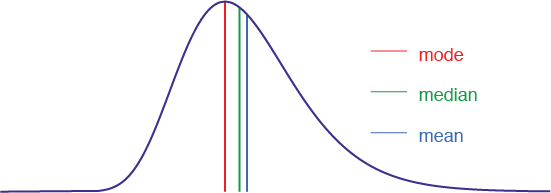
\includegraphics[scale=0.5]{pics/centrales.png}
	
	
\end{figure}
 
\end{frame}







\begin{frame}[fragile]{Percentiles o Cuantiles}
\scriptsize{
\begin{itemize}
 \item El $k$-ésimo percentil de una variable numérica es un valor tal que el $k\%$ de las observaciones se encuentran debajo del percentil y el $(100-k)\%$ se encuentran sobre este valor.
 
 \item En estadística se usan generalmente los \textbf{cuantiles} que son equivalentes a los percentiles expresados en fracciones en vez de porcentajes.
 
 \item En R se calculan con el comando \verb+quantile+:
 \begin{verbatim}
# Todos los percentiles
quantile(Sepal.Length,seq(0,1,0.01))
 \end{verbatim}

 
 \item Además es muy común hablar de los \textbf{cuartiles} que son tres percentiles específicos: 
 
 \begin{itemize}
 \scriptsize{
  \item El primer cuartil $Q_1$ (lower quartile) es el percentil con $k=25$. 
  \item El segundo cuartil $Q_2$ es con  $k=50$  que equivale a la mediana. 
  \item El tercer cuartil $Q_3$ (upper quartile) es con $k=75$.
  }
 \end{itemize}
\begin{verbatim}
# El mínimo, los tres cuartiles y el máximo
> quantile(Sepal.Length,seq(0,1,0.25))
  0%  25%  50%  75% 100% 
 4.3  5.1  5.8  6.4  7.9  
\end{verbatim}

 
\end{itemize}

}

 
\end{frame}


\begin{frame}[fragile]{Resumiendo un Data Frame}
\scriptsize{
\begin{itemize}
 \item En R podemos resumir varias estadísticas de resumen de una variable o de un data.frame usando el comando \verb+summary+.
 \item Para las variables numéricas nos entrega el mínimo, los cuartiles, la media y el máximo. 
 \item Para las variables categóricas nos entrega la tabla de frecuencias.
\end{itemize}


\begin{verbatim}
> summary(iris)
 Sepal.Length    Sepal.Width     Petal.Length    Petal.Width   
 Min.   :4.300   Min.   :2.000   Min.   :1.000   Min.   :0.100  
 1st Qu.:5.100   1st Qu.:2.800   1st Qu.:1.600   1st Qu.:0.300  
 Median :5.800   Median :3.000   Median :4.350   Median :1.300  
 Mean   :5.843   Mean   :3.057   Mean   :3.758   Mean   :1.199  
 3rd Qu.:6.400   3rd Qu.:3.300   3rd Qu.:5.100   3rd Qu.:1.800  
 Max.   :7.900   Max.   :4.400   Max.   :6.900   Max.   :2.500  

 Species  
 setosa    :50  
 versicolor:50  
 virginica :50   
\end{verbatim}

 
} 
\end{frame}


\begin{frame}[fragile]{Ejercicio}
\scriptsize{
\begin{itemize}
 \item Usando el comando \verb+tapply+ analice la media, la mediana y los cuartiles para las tres especies de \textbf{Iris} para las cuatro variables.
 \item ¿Nota alguna diferencia en las distintas especies?
\end{itemize}

\pause

\begin{verbatim}
tapply(iris$Petal.Length,iris$Species,summary)
tapply(iris$Petal.Width,iris$Species,summary)
tapply(iris$Sepal.Length,iris$Species,summary)
tapply(iris$Sepal.Width,iris$Species,summary) 
\end{verbatim}

 
} 
\end{frame}

\begin{frame}[fragile]{Medidas de Dispersión}
\scriptsize{ 
\begin{itemize}
 \item Estas medidas nos dicen que tan distintas o similares tienden a ser las observaciones respecto a un valor particular. Generalmente este valor se refiere a alguna medida de tendencia central.
 \item El rango es la diferencia entre el valor máximo y el mínimo:
 \begin{verbatim}
> max(Sepal.Length)-min(Sepal.Length)
[1] 3.6
 \end{verbatim}
 \item La desviación estándar es la raíz cuadrada de la varianza que mide las diferencias cuadráticas promedio de las observaciones con la media. 
 \begin{displaymath}
  \text{var}(x)=\frac{1}{m-1}\sum_{i=1}^{m}(x_{i} - \overline{x} )^2
 \end{displaymath}
 \begin{displaymath}
  \text{sd}(x)=\sqrt{\text{var}(x)}
 \end{displaymath}

\begin{verbatim}
> var(Sepal.Length)
[1] 0.6856935
> sd(Sepal.Length)
[1] 0.8280661 
\end{verbatim}



\end{itemize}
 
 
 
} 
\end{frame}


\begin{frame}[fragile]{Medidas de Dispersión (2)}
\scriptsize{ 
\begin{itemize}
 \item Al igual que la media, la desviación estándar es sensible a outliers.
 \item Las medidas más robustas se basan generalmente en la mediana.

  \item Sea $m(x)$ una medida de tendencia central de $x$ (usualmente la mediana), se define la \textbf{desviación absoluta promedio} o \textbf{average absolute deviation} (AAD)  como:
  \begin{displaymath}
   \text{AAD}(x) = \frac{1}{m}\sum_{i=1}^{m}|x_i-m(x)| 
  \end{displaymath}
  
  \item Programe la función \verb+add+ en R, como una función que recibe un vector \verb+x+ y una función de media central \verb+fun+. El valor absoluto se calcula con el comando \verb+abs+:
  \pause
  
  \begin{verbatim}
aad<-function(x,fun=median){
  mean(abs(x-fun(x)))
}
> aad(Sepal.Length)
[1] 0.6846667
> aad(Sepal.Length,mean)
[1] 0.6875556
  \end{verbatim}


\end{itemize}
 
 
 
} 
\end{frame}


\begin{frame}[fragile]{Medidas de Dispersión (3)}
\scriptsize{ 
\begin{itemize}
 \item Sea $b$ una constante de escala se define la \textbf{desviación media absoluta} o \textbf{median absolute deviation} como: 
 \begin{displaymath}
  \text{MAD}(x) = b \times \text{median}(|x_{i}-\text{m}(x)|)
 \end{displaymath}
 \item En R se calcula con el comando \verb+mad+ con los parámetros  \verb+center+ como una función que mide la tendencia central de la variable y \verb+constant+ como la constante $b$. Por defecto se usa la mediana y el valor $1.482$. 
 \begin{verbatim}
 > mad(Sepal.Length)
[1] 0.7 
 \end{verbatim}

 \item Finalmente, se define el rango inter-cuartil (IQR) como la diferencia entre el tercer y el primer cuartil ($Q_3 - Q_1$).
 \begin{verbatim}
IQR(Sepal.Length)
[1] 1.3  
 \end{verbatim}

\end{itemize}
  
} 
\end{frame}



\begin{frame}[fragile]{Estadísticas de Resumen Multivariadas}
\scriptsize{
\begin{itemize}
 \item Para comparar como varía una variable  respecto a otra, usamos medidas multivariadas.
 \item La covarianza $cov(x,y)$  mide el grado de variación lineal conjunta de un par de variables $x$, $y$ :
 \begin{displaymath}
  cov(x,y)=\frac{1}{m-1}\sum_{i=1}^{n}(x-\overline{x})(y-\overline{y})
 \end{displaymath}
 \item Donde $cov(x,x)=var(x)$
\item En R se calcula con el comando \verb+cov+:
\begin{verbatim}
> cov(Sepal.Length,Sepal.Width)
[1] -0.042434 
\end{verbatim}
\item Si le damos una matriz o un data.frame de variables numéricas, calcula una matriz de covarianzas:
\begin{verbatim}
> cov(iris[,1:4])
             Sepal.Length Sepal.Width Petal.Length Petal.Width
Sepal.Length    0.6856935  -0.0424340    1.2743154   0.5162707
Sepal.Width    -0.0424340   0.1899794   -0.3296564  -0.1216394
Petal.Length    1.2743154  -0.3296564    3.1162779   1.2956094
Petal.Width     0.5162707  -0.1216394    1.2956094   0.5810063 
\end{verbatim}

 
 
\end{itemize}



}
\end{frame}


\begin{frame}[fragile]{Estadísticas de Resumen Multivariadas (2)}
\scriptsize{
\begin{itemize}
 \item Si dos variables son independientes entre sí, su covarianza es cero.
 \item Para tener una medida de relación que no dependa de la escala de cada variable, usamos la \textbf{correlación lineal}.
 \item Se define a la correlación lineal o coefiente de correlación de \textbf{Pearson} $r(x,y)$ como:
 \begin{displaymath}
  r(x,y)=\frac{cov(x,y)}{sd(x)sd(y)}
 \end{displaymath}
\item La correlación lineal varía entre $-1$ a $1$. Un valor cercano a 1 indica que mientras una variable crece  la otra también lo hace en una proporción lineal. Un valor cercano a -1 indica una relación inversa (una crece la otra decrece). Si la correlación es cercana a cero tenemos independencia lineal. Ojo que eso no implica que no pueda haber una relación no-lineal entre las variables.
\item En R se calcula con el comando \verb+cor+.
\begin{verbatim}
> cor(iris[,1:4])
             Sepal.Length Sepal.Width Petal.Length Petal.Width
Sepal.Length    1.0000000  -0.1175698    0.8717538   0.8179411
Sepal.Width    -0.1175698   1.0000000   -0.4284401  -0.3661259
Petal.Length    0.8717538  -0.4284401    1.0000000   0.9628654
Petal.Width     0.8179411  -0.3661259    0.9628654   1.0000000
\end{verbatim}

 
 
\end{itemize}



}
\end{frame}


\begin{frame}[fragile]{Tablas de Contingencia}
\scriptsize{
\begin{itemize}
 \item Para analizar la relación entre variables de naturaleza categórica usamos \textbf{tablas de contingencia}.
 \item La tabla se llena con las frecuencias marginales de todos los pares de valores entre dos variables categóricas.
 \item En R se crean usando el comando \verb+table+ que usábamos para frecuencias, pero entregándole dos vectores:
 \begin{verbatim}
sexo<-c("Hombre","Hombre","Mujer","Hombre","Mujer","Mujer")
estudios<-c("universitario","secundario","secundario",
            "postgrado","secundario","universitario")
            
> table(sexo,estudios)
        estudios
sexo     postgrado secundario universitario
  Hombre         1          1             1
  Mujer          0          2             1    
 \end{verbatim}

 
 
\end{itemize}


} 
\end{frame}





%%% Tablas de contingencia
%%% Correlaciones

\section{Visualización}


\begin{frame}[fragile]{Visualización de Datos}
\scriptsize{
\begin{itemize}
 \item La visualización de datos es la transformación de un dataset a un formato visual que permita a las personas identificar las características y las relaciones entre los elementos del dataset.
 
 \item La visualización permite que las personas reconozcan patrones o tendencias en base a su criterio o expertiz en el dominio particular.
 
   \begin{figure}[h!]
	\centering
	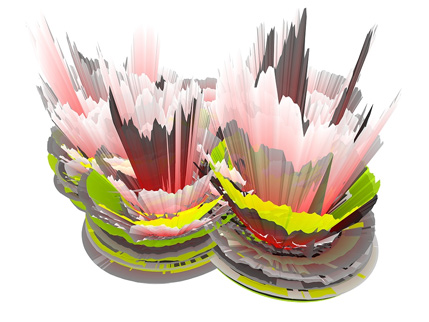
\includegraphics[scale=0.38]{pics/visua.jpg}
	
	
\end{figure} 
 
\end{itemize}

}
 
\end{frame}

\begin{frame}{Representación}
\scriptsize{
\begin{itemize}
 \item Se entiende por representación como el mapeo que se hace a partir de los datos hacia un formato visual.
 \item Se traducen los datos, sus atributos y relaciones a elementos gráficos como puntos, líneas, formas y colores. 
  \item Los objetos son usualmente representados como puntos.
  \item Los valores de atributos se representan como la posición de los puntos o las características de los puntos, ej: color, tamaño y forma.
  \item Cuando se usa la posición para representar los valores es simple detectar si es que se forman grupos de obejtos o la presencia de objetos atípicos. 
  
 
 
\end{itemize}
 
 

 
}
\end{frame}


\begin{frame}[fragile]{Graficando en R}
\scriptsize{
\begin{itemize}
 \item  En R la función de visualización más frecuente en \verb+plot+. 
 \item Es una función genérica cuyo resultado depende de la naturaleza de las variables usadas. 
 
 \item  A todos los gráficos les podemos agregar parámetros adicionales como: \verb+main+ para el título, \verb+xlab+ e \verb+ylab+  para el nombre del eje x y del el eje y.
 
 \item Otras propiedades son \verb+col+ para definir el color, \verb+type+ para definir el tipo de gráfico: (p) para puntos o (l) para líneas.
 
 \item Además podemos agregarle nuevas capas a un gráfico con el comando \verb+lines+.
 
 \item Para grabar una imagen en un archivo podemos usar el botón \textbf{export} de Rstudio.
 
 \item Para hacerlo de la línea de comandos en R:
 \begin{verbatim}
png("imagen.png")
plot(1:10)
dev.off() 
 \end{verbatim}

 


 
 
\end{itemize}


 
} 
\end{frame}


\begin{frame}[fragile]{Ejemplo}
\scriptsize{
  \begin{verbatim}
plot(rnorm(15,10,5),col="red",type="l")
lines(rnorm(15,10,5),col="blue",type="p",pch=1)
lines(rnorm(15,10,5),col="green",type="b",pch=2)
title(main="Mi gráfico")
legend('topright', c("lineas","puntos","ambos") , 
       lty=1:3, col=c("red", "blue","green"), bty='n', cex=.75)  
 \end{verbatim}
 
 
  \begin{figure}[h!]
	\centering
	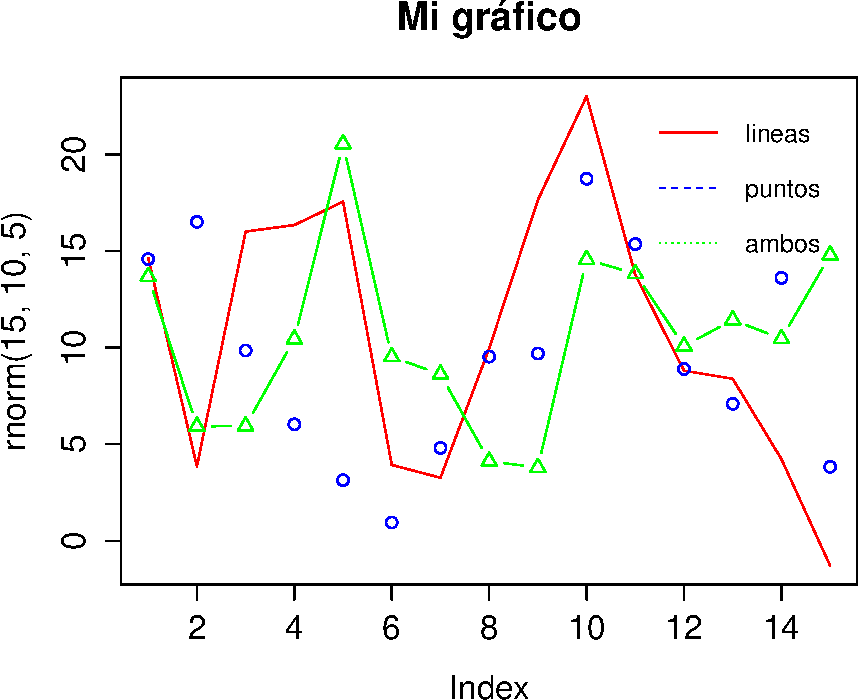
\includegraphics[scale=0.38]{pics/rplot.pdf}
	
	
\end{figure} 



 
} 
\end{frame}



\begin{frame}[fragile]{Histogramas}
\scriptsize{
\begin{itemize}
 \item Muestran la distribución de los valores de una variable.
 \item Los valores de los elementos se dividen en contenedores (bins) y se crean gráficos de barra por cada contenedor.
 \item La altura de cada barra indica el número de elementos o frecuencia del contenedor.
 \item En R se crean con el comando \verb+hist+.
 \begin{verbatim}
> hist(Sepal.Length)
 \end{verbatim}
 \begin{figure}[h!]
	\centering
	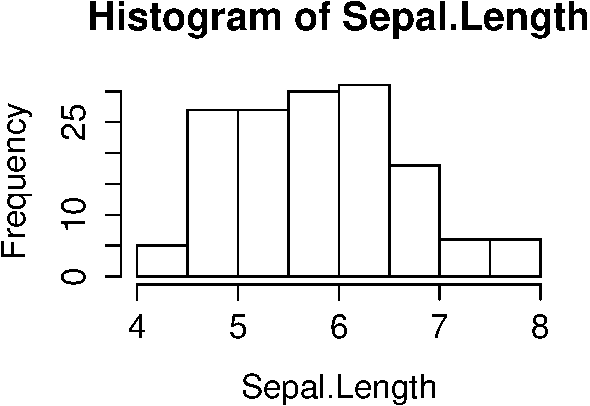
\includegraphics[scale=0.6]{pics/hist1.pdf}
	
	
\end{figure} 

\end{itemize}




}
\end{frame}


\begin{frame}[fragile]{Histogramas (2) }
\scriptsize{
\begin{itemize}
 \item La forma del histograma depende de el número de contenedores.
 \item En R se puede definir esa cantidad con el parámetro \verb+nclass+.
 \begin{verbatim}
> hist(Sepal.Length,nclass=100)
 \end{verbatim}
 \begin{figure}[h!]
	\centering
	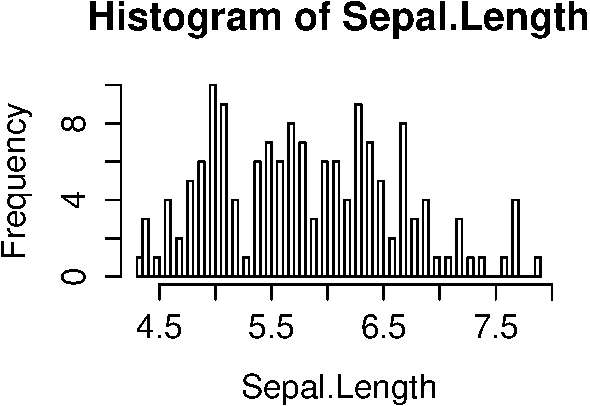
\includegraphics[scale=0.6]{pics/hist2.pdf}
	
	
\end{figure} 

\end{itemize}

}
\end{frame}


\begin{frame}[fragile]{Histogramas (3) }
\scriptsize{
\begin{itemize}
 \item Una librería muy popular para hacer visualizaciones en R es \emph{ggplot2}.
 \item Se basa en la idea de descomponer el gráfico en componentes semánticos como escalas y capas.
 
 \begin{verbatim}
>install.packages("ggplot2")
>library(ggplot2)
>ggplot(iris, aes(x=Sepal.Length)) 
+ geom_histogram(bins = 10, color="black", fill="white")
 \end{verbatim}
 \begin{figure}[h!]
	\centering
	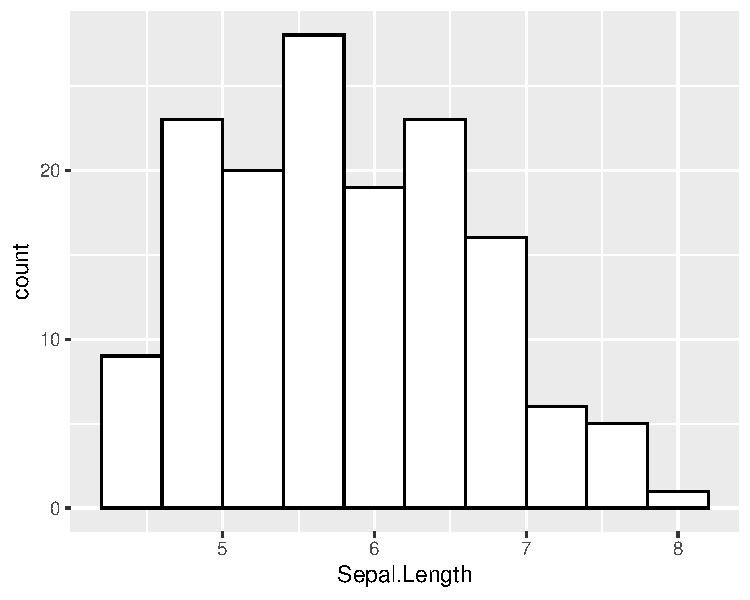
\includegraphics[scale=0.4]{pics/hist3.pdf}
	
	
\end{figure} 

\end{itemize}

}
\end{frame}


\begin{frame}[fragile]{Densidad }
\scriptsize{
\begin{itemize}
 \item Otra forma de visualizar como se distribuyen los datos es estimando una densidad.
 \item Se calculan usando técnicas estadísticas no paramétricas llamadas estimación de densidad de \textbf{kernel}.
 \item La densidad es una versión suavizada del histograma y nos permite determinar más claramente si los datos observados se comportan como una densidad conocida ej: normal. 
 \item En R se crean con el comando \verb+density+, para luego visualizarlas con el comando \verb+plot+.

 \begin{verbatim}
plot(density(iris$Sepal.Length),main="Densidad de Sepal.Length")
 \end{verbatim}
 \begin{figure}[h!]
	\centering
	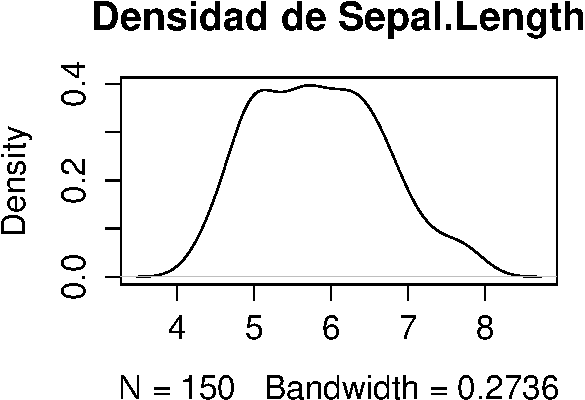
\includegraphics[scale=0.5]{pics/density.pdf}
	
	
\end{figure} 

\end{itemize}




}
\end{frame}


\begin{frame}[fragile]{Gráficos de Torta o Pie Charts }
\scriptsize{
\begin{itemize}
 \item Los gráficos de torta, gráficos circulares o pie charts representan la frecuencia de los elementos en un círculo.
 \item Cada elemento tiene una participación proporcional a su frecuencia relativa.
 \item Se usan generalmente para variables categóricas:
 \begin{verbatim}
pie(table(iris$Species))
 \end{verbatim}
 \begin{figure}[h!]
	\centering
	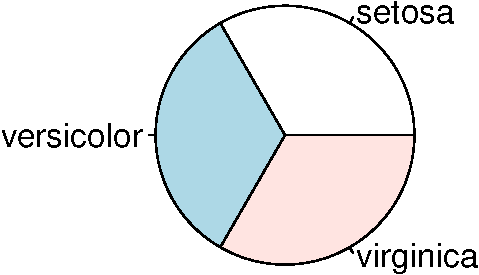
\includegraphics[scale=0.6]{pics/piechart.pdf}
	
	
\end{figure} 

\end{itemize}




}
\end{frame}


\begin{frame}[fragile]{Boxplots}
\scriptsize{
\begin{itemize}
 \item Los Boxplots o diagramas de caja se construyen a partir de los percentiles. 
 \item Se construye una rectángulo usando entre el primer y el tercer cuartil ($Q_1$ y $Q_3$).
 \item La altura del rectángulo es el rango intercuartil RIC ($Q_3 - Q_1$).
 \item La mediana es una línea que divide el rectángulo.
 \item Cada extremo del rectángulo se extiende con una recta o brazos de largo $Q1-1.5*$RIC para la recta inferior y  $Q_3+1.5*$RIC para la recta superior.
 \item Los valores más extremos que el largo de los brazos son considerados atípicos.
 
 \item El boxplot nos entrega información sobre la simetría de la distribución de los datos.
  \item Si la mediana no está en el centro del rectángulo, la distribución no es simétrica.
 \item Son útiles para ver la presencia de valores atípicos u outliers.
 
\end{itemize}



}
\end{frame}


\begin{frame}{Boxplots (2)}
\begin{figure}[h!]
	\centering
	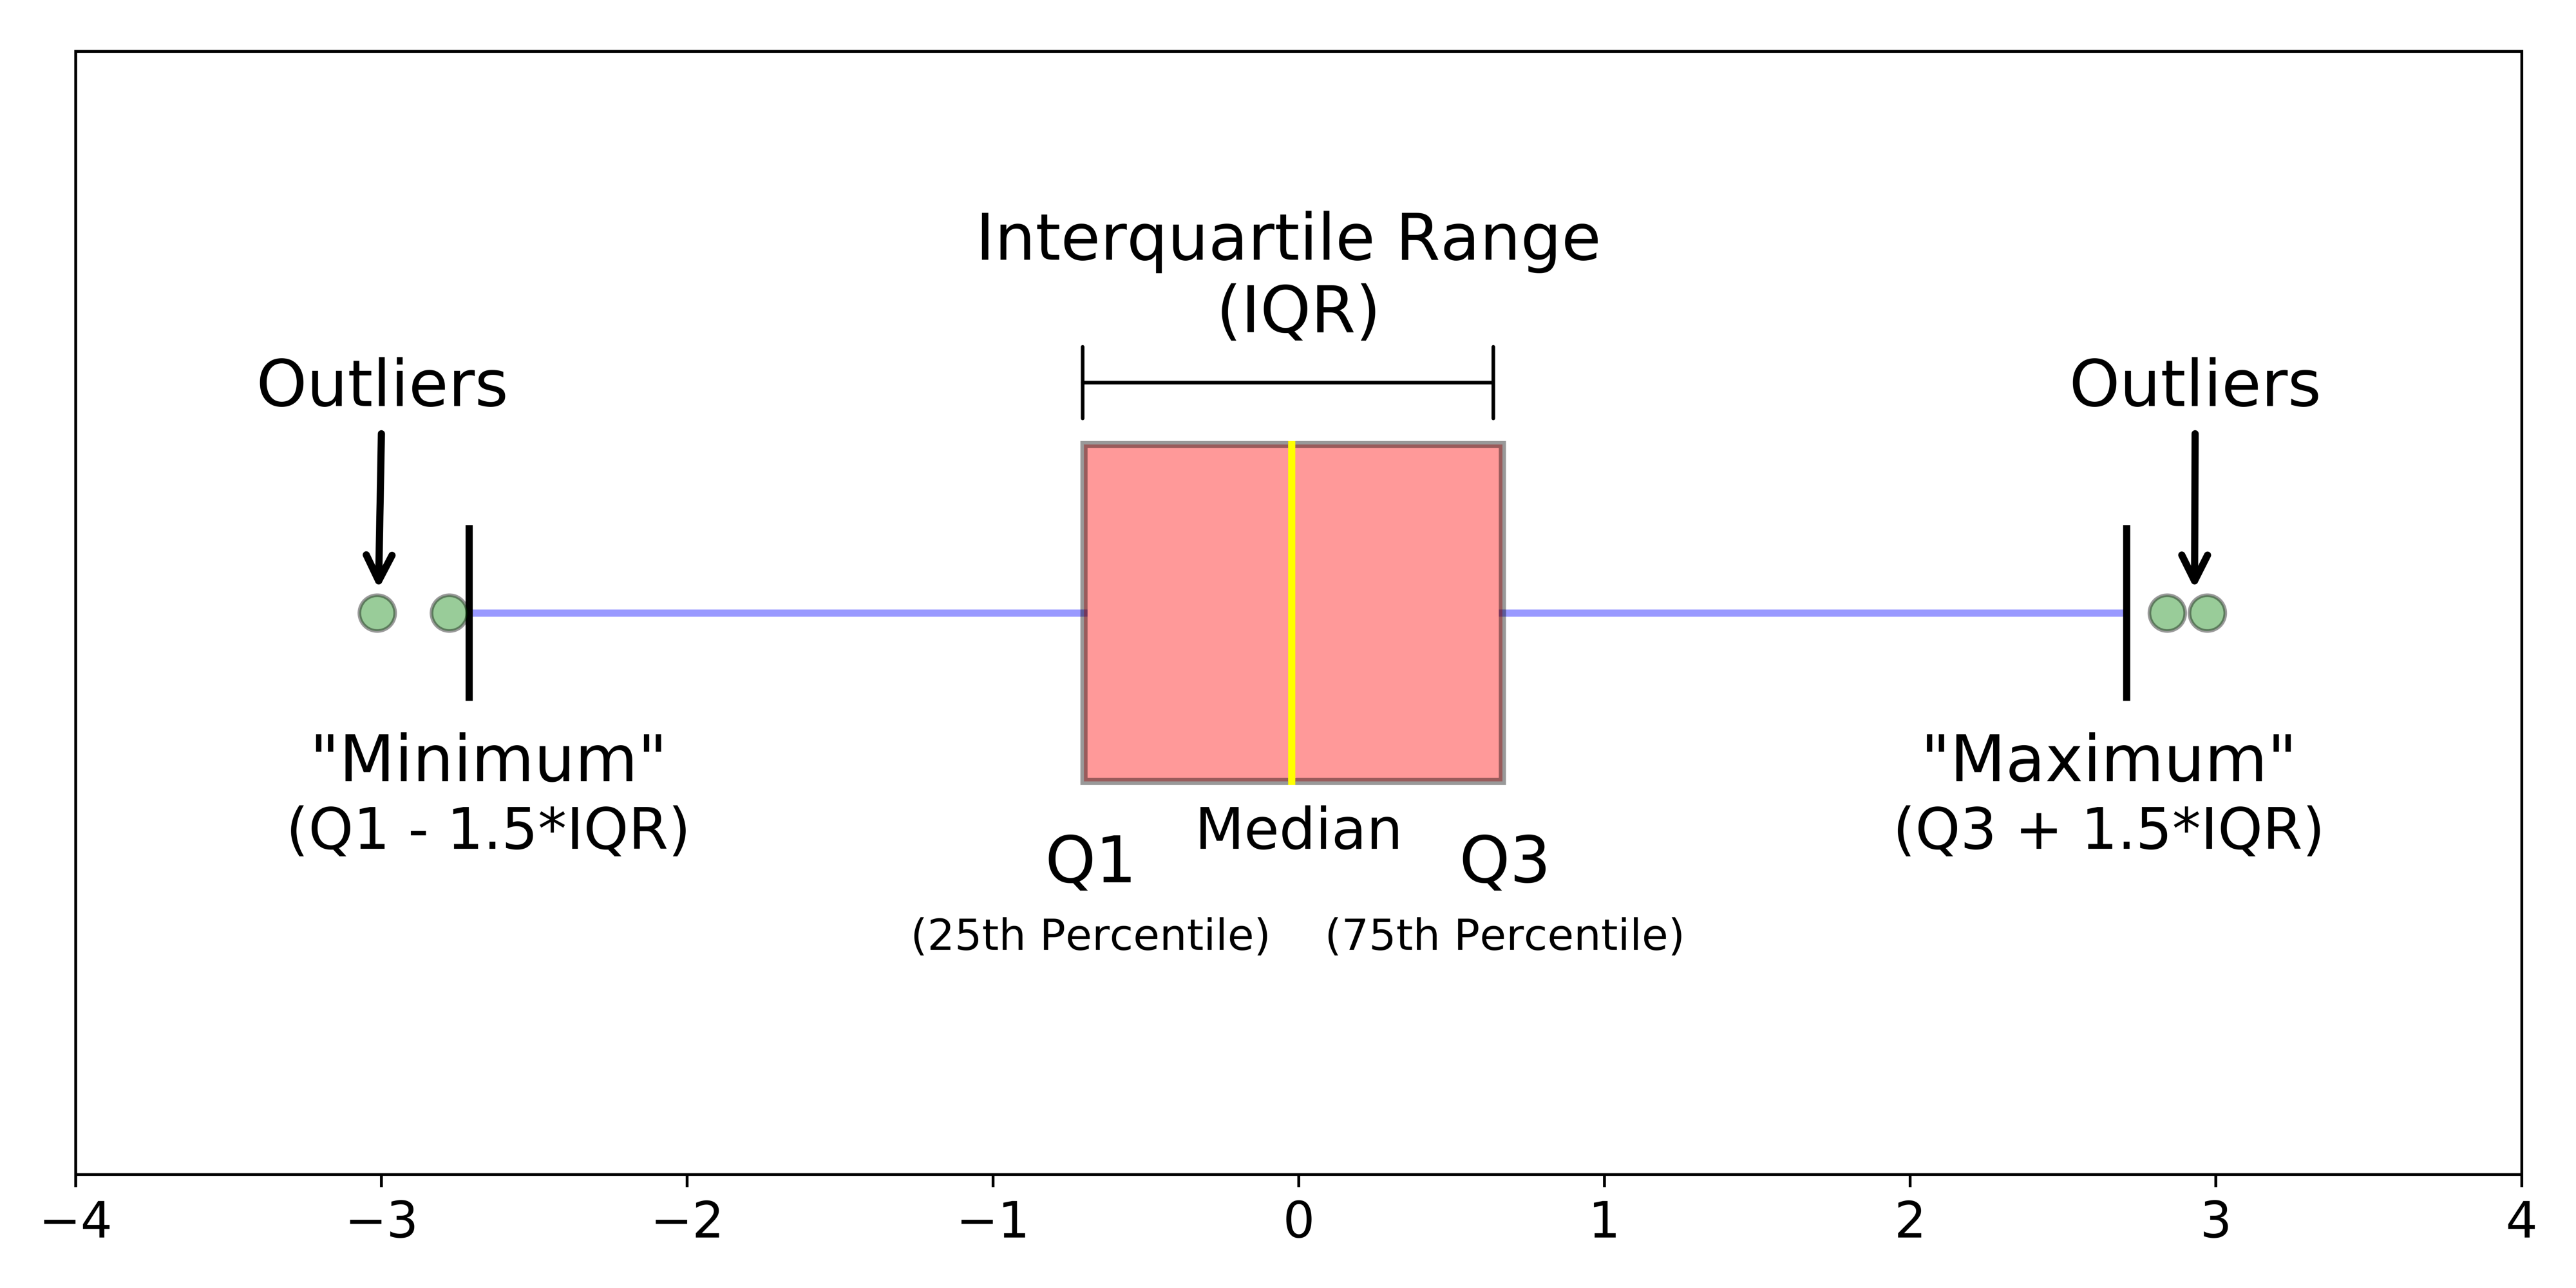
\includegraphics[scale=0.35]{pics/boxplot.png}
	\caption{Fuente: \url{http://commons.wikimedia.org/wiki/File:Boxplot.svg}}
	
\end{figure} 
\end{frame}


\begin{frame}{Boxplots (3)}
\scriptsize{
\begin{itemize}
 \item El largo de los brazos así como el criterio para identificar valores atípicos se basa en el comportamiento de una normal.
\end{itemize}

\begin{figure}[h!]
	\centering
	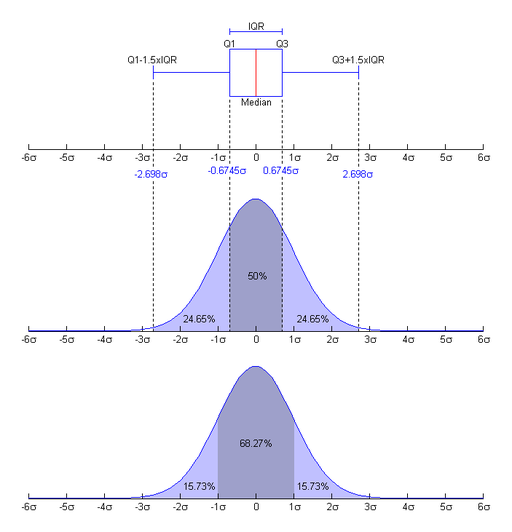
\includegraphics[scale=0.35]{pics/Boxplot_vs_PDF.png}
	
	
	
\end{figure} 
}
\end{frame}

\begin{frame}[fragile]{Boxplots (4)}
\scriptsize{
\begin{itemize}
 \item En R los boxplots se grafican con el comando \verb+boxplot+:
 \begin{verbatim}
> boxplot(Sepal.Length,main="Boxplot Sepal.Length")
 \end{verbatim}

 \begin{figure}[h!]
	\centering
	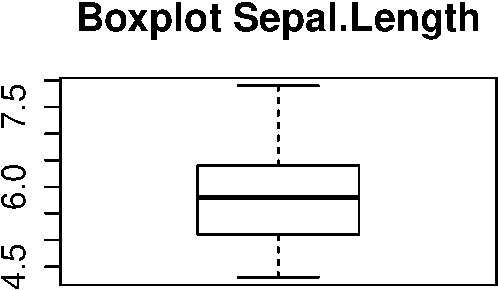
\includegraphics[scale=0.7]{pics/boxplotsimple.pdf}		
\end{figure} 
 
 
\end{itemize}



}
\end{frame}


\begin{frame}[fragile]{Boxplots (4)}
\scriptsize{
\begin{itemize}

\item Si tenemos una variable factor podemos crear un boxplot para cada categoría de la siguiente manera:
\begin{verbatim}
> boxplot(Sepal.Length~Species,ylab="Sepal.Length")
\end{verbatim}

 \begin{figure}[h!]
	\centering
	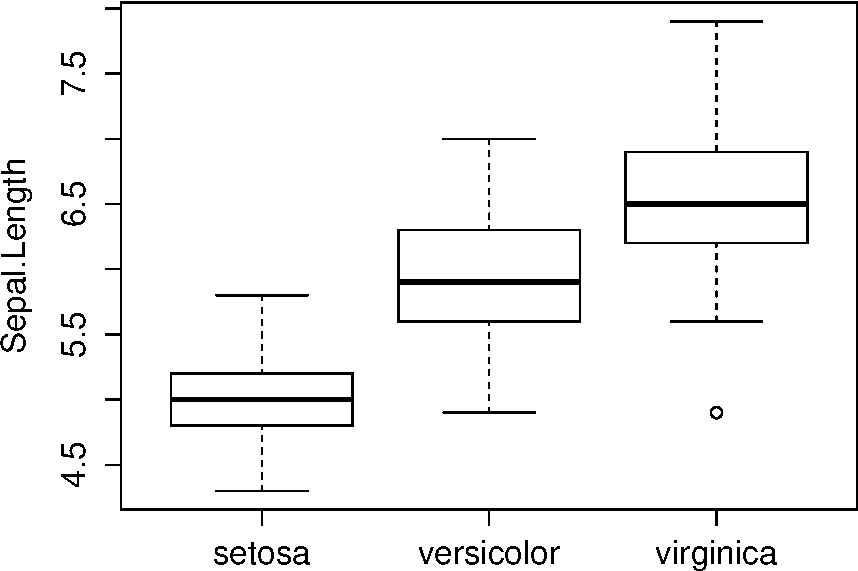
\includegraphics[scale=0.5]{pics/boxplotfactor.pdf}		
\end{figure} 
 
\end{itemize}

}
\end{frame}
\begin{frame}[fragile]{Boxplots (5)}
\scriptsize{
\begin{itemize}

\item También podemos podemos comparar varios boxplots en un mismo gráfico:
\begin{verbatim}
> boxplot(x=iris[,1:4],main="Boxplots Iris")
\end{verbatim}

 \begin{figure}[h!]
	\centering
	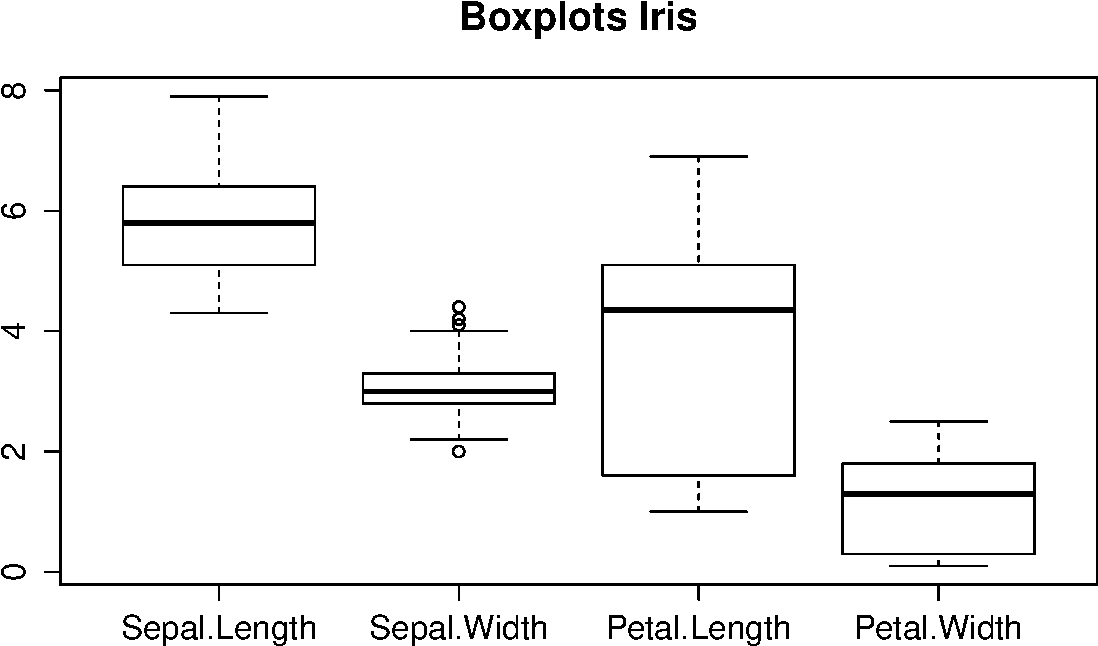
\includegraphics[scale=0.5]{pics/boxplotiris.pdf}		
\end{figure} 
 
\end{itemize}

}
\end{frame}



\begin{frame}[fragile]{Boxplots (6)}
\scriptsize{
\begin{itemize}

\item Ahora usando \emph{ggplot2}:
\begin{verbatim}
> ggplot(iris, aes(x = Species, y = Sepal.Length, 
  fill = Species)) +  geom_boxplot()
\end{verbatim}

 \begin{figure}[h!]
	\centering
	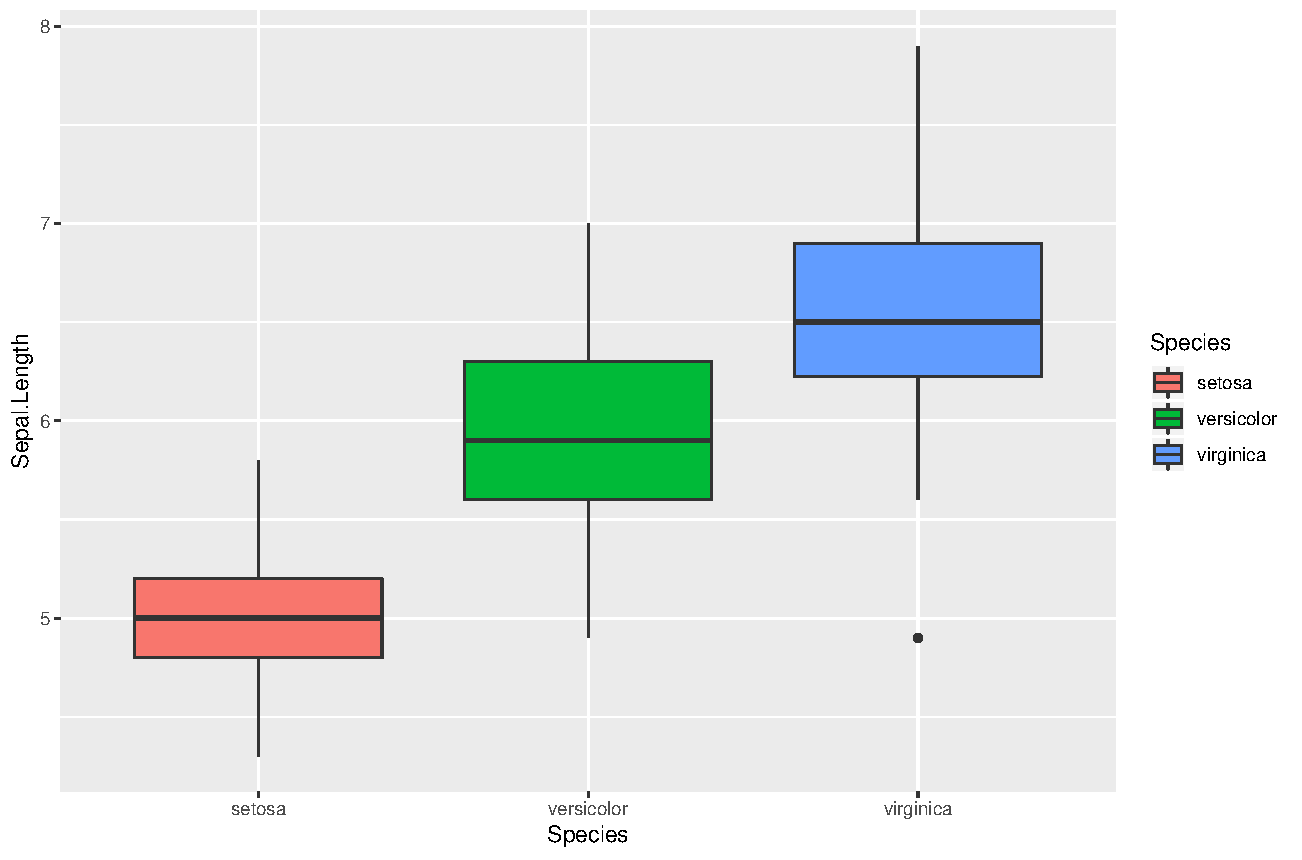
\includegraphics[scale=0.4]{pics/boxplotggplot2.pdf}		
\end{figure} 
 
\end{itemize}

}
\end{frame}


\begin{frame}[fragile]{Diagramas de Dispersión}
\scriptsize{
\begin{itemize}
 \item Los diagramas de dispersión o scatter plots usan coordenadas cartesianas para mostrar los valores de dos variables númericas del mismo largo.
 \item Los valores de los atributos determinan la posición de los elementos.
 \item Otros atributos pueden usarse para definir el tamaño, la forma o el color de los objetos.
 
  \item En R podemos graficar un scatterplot de dos variables numéricas usando el comando \verb+plot(x,y)+, que sería $y$ vs $x$.
  \item También se pueden definir fórmulas $f(x)=y$  usando la notación \verb+y~x+. 
  
 \item De esta manera el comando \verb+plot(y~x)+ es equivalente a \verb+plot(x,y)+.
 
 \item Si tenemos un data.frame o matriz numérica podemos ver los scatterplots de todos los pares usando el comando \verb+pairs(x)+.
  
 
 
\end{itemize}




}
 
\end{frame}


\begin{frame}[fragile]{Diagramas de Dispersión (2)}
\scriptsize{
\begin{itemize}
 \item Ejemplos:
 \begin{verbatim}
# El ancho del sépalo vs el largo del sépalo  
plot(Sepal.Width~Sepal.Length, col=Species)
# Equivalente
plot(Sepal.Length, Sepal.Width,col=Species,
     pch=as.numeric(Species))
# Le agregamos una leyenda
legend('topright', levels(Species) , 
       lty=1, col=1:3, bty='n', cex=.75)  
 \end{verbatim}

  \begin{figure}[h!]
	\centering
	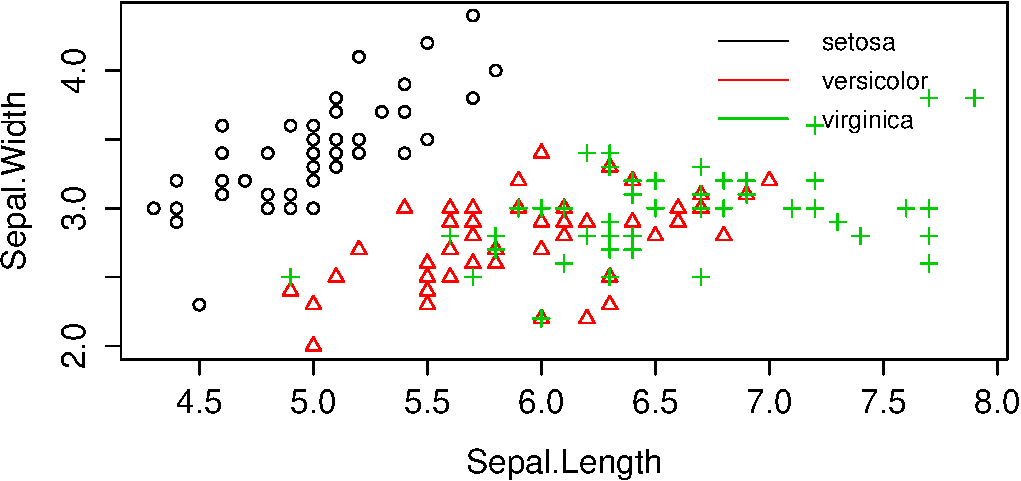
\includegraphics[scale=0.5]{pics/scatter1.pdf}		
\end{figure} 
 
 
\end{itemize}




}
 
\end{frame}


\begin{frame}[fragile]{Diagramas de Dispersión (3)}
\scriptsize{
\begin{itemize}
 \item Lo mismo usando \emph{ggplot2}:
 \begin{verbatim}
ggplot(iris, aes(x=Sepal.Length,
y=Sepal.Width, color=Species)) + 
geom_point(size=3,shape=4)
 \end{verbatim}

  \begin{figure}[h!]
	\centering
	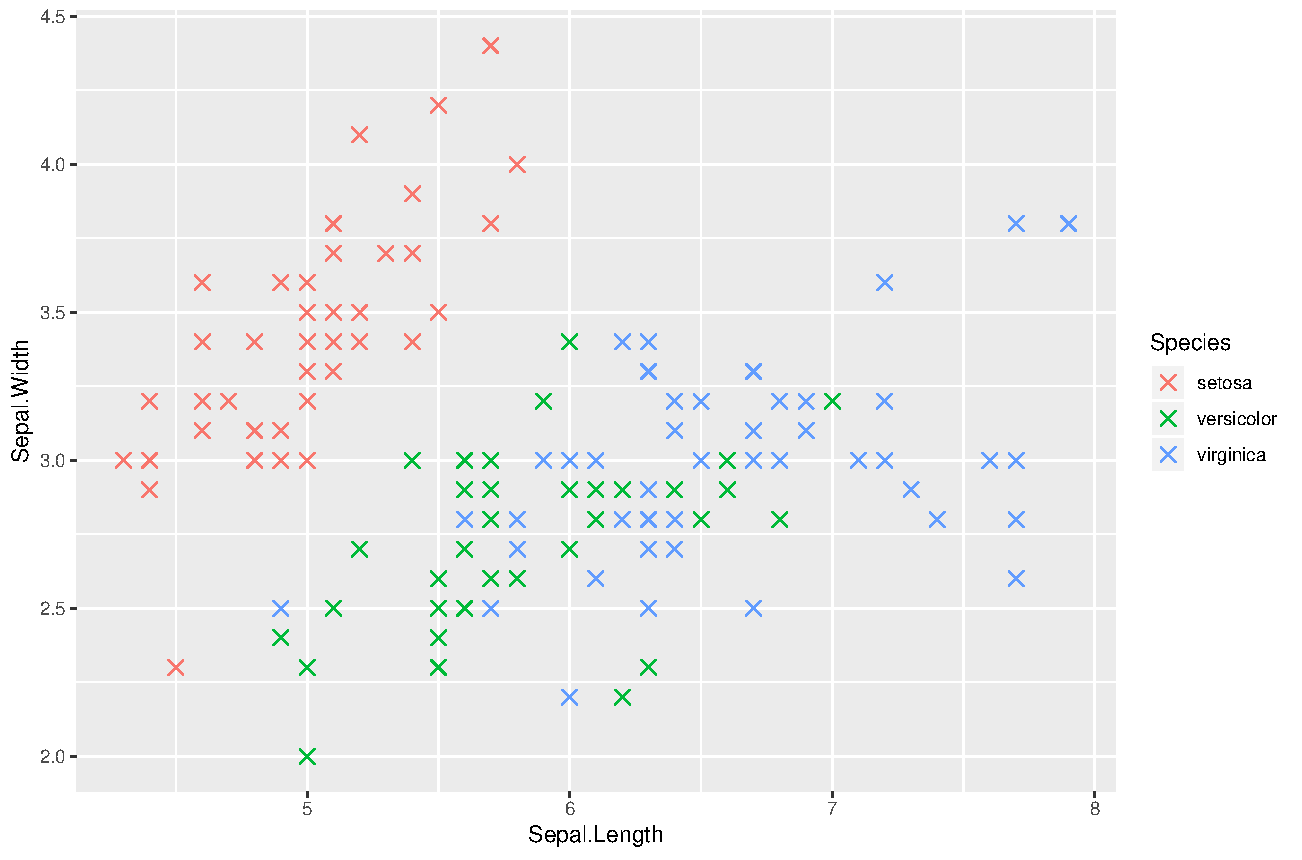
\includegraphics[scale=0.4]{pics/scatterggplot2.pdf}		
\end{figure} 
 
 
\end{itemize}




}
\end{frame}


\begin{frame}[fragile]{Diagramas de Dispersión (4)}
\scriptsize{
\begin{itemize}
 \item Todos los pares de las 4 variables del dataset iris usando un color y un carácter distinto para cada especie:
 \begin{verbatim}
pairs(iris[,1:4],pch=as.numeric(iris$Species),col=iris$Species)
 \end{verbatim}

  \begin{figure}[h!]
	\centering
	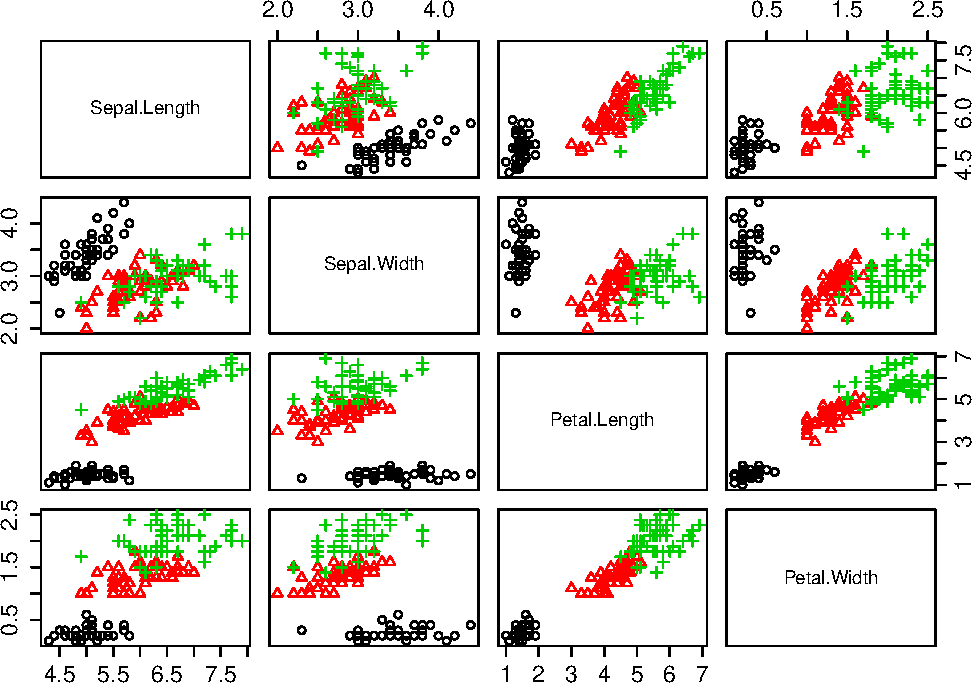
\includegraphics[scale=0.5]{pics/scatter2.pdf}		
\end{figure} 
 
 
\end{itemize}

}
 
\end{frame}


\begin{frame}[fragile]{Diagramas de Dispersión (5)}
\scriptsize{
\begin{itemize}
 \item También se pueden crear scatterplots en tres dimensiones.
 \item Se debe instalar la librería \verb+scatterplot3d+ usando el siguiente comando:
 
 \begin{verbatim}
 install.packages("scatterplot3d",dependencies=T)
 \end{verbatim}
 
 \item Luego cargan la librería escribiendo \verb+library(scatterplot3d)+.
 
 \item Un scatterplot 3d para el ancho del pétalo, el largo del sépalo y el ancho del sépalo:
 \begin{verbatim}
scatterplot3d(iris$Petal.Width, iris$Sepal.Length, 
              iris$Sepal.Width, color=as.numeric(iris$Species),
              pch=as.numeric(iris$Species))  
 \end{verbatim}

 
  
\end{itemize}




}
 
\end{frame}


\begin{frame}[fragile]{Diagramas de Dispersión (6)}

 
 
  \begin{figure}[h!]
	\centering
	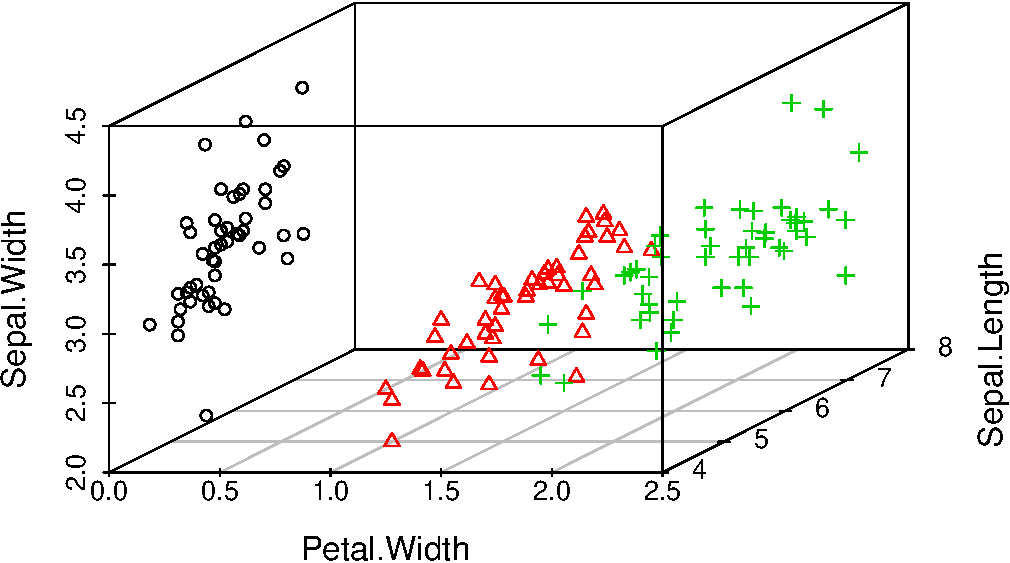
\includegraphics[scale=0.6]{pics/scatter3.pdf}		
\end{figure} 
 
 

 
\end{frame}



\begin{frame}[fragile]{Gráficos de Coordenadas Paralelas}
\scriptsize{
 \begin{itemize}
  \item Los gráficos de coordenadas paralelas son otra forma de visualizar datos multi-dimensionales.
  \item En vez de usar ejes perpendiculares (x-y-z) usamos varios ejes paralelos entre sí.
  \item Cada atributo es representado por uno de los ejes paralelo con sus respectivos valores.
  \item Los valores de los distintos atributos son escalados para que cada eje tenga la misma altura.
  \item Cada observación representa una línea que une los distintos ejes de acuerdo a sus valores.
  \item De esta manera, objetos similares entre sí tienden a agruparse en líneas con trayectoria similar.
  \item En muchas ocasiones es necesario realizar un re-ordenamiento de los ejes para poder visualizar un patrón.
 \end{itemize} 
 
 }  
\end{frame}


\begin{frame}[fragile]{Gráficos de Coordenadas Paralelas (2)}
\scriptsize{
 \begin{itemize}
  \item En R podemos crear gráficos de coordenadas paralelas con el comando \verb+parcoord+ de la librería \verb+MASS+.
  \item Ejemplo:
  \begin{verbatim}
library(MASS)
parcoord(iris[1:4], col=iris$Species,var.label=T)   
  \end{verbatim}
  
  \begin{figure}[h!]
	\centering
	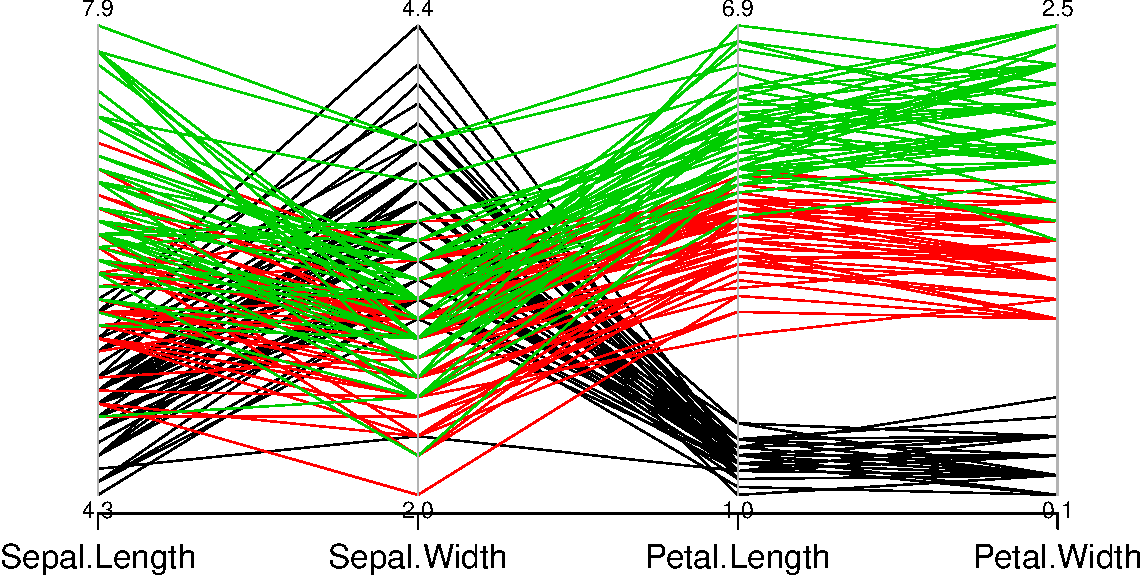
\includegraphics[scale=0.5]{pics/parallel.pdf}		
\end{figure}   

 \end{itemize} 
 
 }  
\end{frame}



\begin{frame}[fragile]{Otras técnicas de Visualización}
\scriptsize{
\begin{block}{Gráficos de Estrellas}
\begin{itemize}
  \item También conocidos como \textbf{gráficos radiales}.
  \item Cada estrella representa una observación, formando un polígono a partir de cada variables con dirección a las agujas del reloj hasta formar un polígono.
  \item El tamaño de cada línea respecto al centro de la estrella corresponde al valor re-escalado de la variable.
  \item Sirve para comparar objetos o detectar valores atípicos.
  \end{itemize} 
  
\end{block}

\begin{block}{Caras de Chernoff}
\begin{itemize}
 \item Enfoque creado por Herman Chernoff basado en la capacidad humana para distinguir rostros. 
 \item Cada atributo corresponde a alguna característica de la cara (boca, ojos, nariz, etc..)
 \item El valor de los atributos determina la apariencia de la característica facial.
 \item Cada observación es una cara.
\end{itemize}
 
 
\end{block}


 
 }  
\end{frame}

\begin{frame}[fragile]{Ejemplo Star Plot}
\scriptsize{
\begin{verbatim}
iris_sample1<-iris[sample(1:dim(iris)[1],size=6,replace=F),]
rownames(iris_sample1)<-paste(as.character(iris_sample1$Species),1:6)
stars(iris_sample1[1:4]) 
\end{verbatim}

  \begin{figure}[h!]
	\centering
	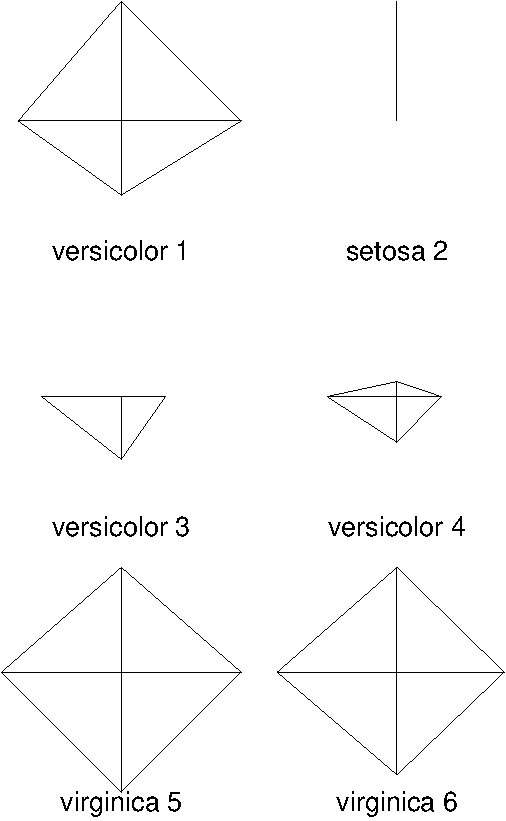
\includegraphics[scale=0.4]{pics/star.pdf}		
\end{figure}   




}
 
\end{frame}


\begin{frame}[fragile]{Ejemplo Chernoff Face}
\scriptsize{
\begin{verbatim}
library("aplpack")
iris_sample<-iris[sample(1:dim(iris)[1],size=16,replace=F),]
faces(iris_sample[1:4],face.type=1,labels=iris_sample$Species)
\end{verbatim}

  \begin{figure}[h!]
	\centering
	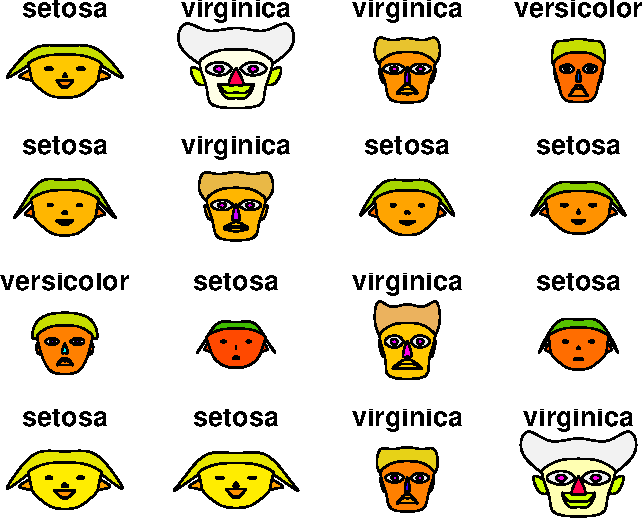
\includegraphics[scale=0.6]{pics/faces.pdf}		
\end{figure}   




}
 
\end{frame}



%%%%%%%%%%%%%%%%%%%%%%%%%%%
\begin{frame}[allowframebreaks]\scriptsize
\frametitle{Bilbiografía}
%\bibliography{bio}
%\bibliographystyle{apalike}
\begin{thebibliography}{8}

\bibitem{William}
Venables, William N., David M. Smith, and R Development Core Team. \emph{An introduction to R.}, 2002.
\bibitem{Pang}
Tan, P. N., Steinbach, M., \& Kumar, V. \emph{Introduction to Data Mining}, 2005.

\bibitem{cran}
\url{http://cran.r-project.org/doc/contrib/grafi3.pdf}
\end{thebibliography}


%\bibliographystyle{flexbib}
\end{frame}










%%%%%%%%%%%%%%%%%%%%%%%%%%%

\end{document}
